
%% bare_conf.tex
%% V1.3
%% 2007/01/11
%% by Michael Shell
%% See:
%% http://www.michaelshell.org/
%% for current contact information.
%%
%% This is a skeleton file demonstrating the use of IEEEtran.cls
%% (requires IEEEtran.cls version 1.7 or later) with an IEEE conference paper.
%%
%% Support sites:
%% http://www.michaelshell.org/tex/ieeetran/
%% http://www.ctan.org/tex-archive/macros/latex/contrib/IEEEtran/
%% and
%% http://www.ieee.org/

%%*************************************************************************
%% Legal Notice:
%% This code is offered as-is without any warranty either expressed or
%% implied; without even the implied warranty of MERCHANTABILITY or
%% FITNESS FOR A PARTICULAR PURPOSE! 
%% User assumes all risk.
%% In no event shall IEEE or any contributor to this code be liable for
%% any damages or losses, including, but not limited to, incidental,
%% consequential, or any other damages, resulting from the use or misuse
%% of any information contained here.
%%
%% All comments are the opinions of their respective authors and are not
%% necessarily endorsed by the IEEE.
%%
%% This work is distributed under the LaTeX Project Public License (LPPL)
%% ( http://www.latex-project.org/ ) version 1.3, and may be freely used,
%% distributed and modified. A copy of the LPPL, version 1.3, is included
%% in the base LaTeX documentation of all distributions of LaTeX released
%% 2003/12/01 or later.
%% Retain all contribution notices and credits.
%% ** Modified files should be clearly indicated as such, including  **
%% ** renaming them and changing author support contact information. **
%%
%% File list of work: IEEEtran.cls, IEEEtran_HOWTO.pdf, bare_adv.tex,
%%                    bare_conf.tex, bare_jrnl.tex, bare_jrnl_compsoc.tex
%%*************************************************************************

% *** Authors should verify (and, if needed, correct) their LaTeX system  ***
% *** with the testflow diagnostic prior to trusting their LaTeX platform ***
% *** with production work. IEEE's font choices can trigger bugs that do  ***
% *** not appear when using other class files.                            ***
% The testflow support page is at:
% http://www.michaelshell.org/tex/testflow/



% Note that the a4paper option is mainly intended so that authors in
% countries using A4 can easily print to A4 and see how their papers will
% look in print - the typesetting of the document will not typically be
% affected with changes in paper size (but the bottom and side margins will).
% Use the testflow package mentioned above to verify correct handling of
% both paper sizes by the user's LaTeX system.
%
% Also note that the "draftcls" or "draftclsnofoot", not "draft", option
% should be used if it is desired that the figures are to be displayed in
% draft mode.
%
\documentclass[conference, letterpaper]{IEEEtran}
% Add the compsoc option for Computer Society conferences.
%
% If IEEEtran.cls has not been installed into the LaTeX system files,
% manually specify the path to it like:
% \documentclass[conference]{../sty/IEEEtran}





% Some very useful LaTeX packages include:
% (uncomment the ones you want to load)

\usepackage{listings}

% *** MISC UTILITY PACKAGES ***
%
%\usepackage{ifpdf}
% Heiko Oberdiek's ifpdf.sty is very useful if you need conditional
% compilation based on whether the output is pdf or dvi.
% usage:
% \ifpdf
%   % pdf code
% \else
%   % dvi code
% \fi
% The latest version of ifpdf.sty can be obtained from:
% http://www.ctan.org/tex-archive/macros/latex/contrib/oberdiek/
% Also, note that IEEEtran.cls V1.7 and later provides a builtin
% \ifCLASSINFOpdf conditional that works the same way.
% When switching from latex to pdflatex and vice-versa, the compiler may
% have to be run twice to clear warning/error messages.






% *** CITATION PACKAGES ***
%
%\usepackage{cite}
% cite.sty was written by Donald Arseneau
% V1.6 and later of IEEEtran pre-defines the format of the cite.sty package
% \cite{} output to follow that of IEEE. Loading the cite package will
% result in citation numbers being automatically sorted and properly
% "compressed/ranged". e.g., [1], [9], [2], [7], [5], [6] without using
% cite.sty will become [1], [2], [5]--[7], [9] using cite.sty. cite.sty's
% \cite will automatically add leading space, if needed. Use cite.sty's
% noadjust option (cite.sty V3.8 and later) if you want to turn this off.
% cite.sty is already installed on most LaTeX systems. Be sure and use
% version 4.0 (2003-05-27) and later if using hyperref.sty. cite.sty does
% not currently provide for hyperlinked citations.
% The latest version can be obtained at:
% http://www.ctan.org/tex-archive/macros/latex/contrib/cite/
% The documentation is contained in the cite.sty file itself.






% *** GRAPHICS RELATED PACKAGES ***
%
\ifCLASSINFOpdf
  % \usepackage[pdftex]{graphicx}
  % declare the path(s) where your graphic files are
  % \graphicspath{{../pdf/}{../jpeg/}}
  % and their extensions so you won't have to specify these with
  % every instance of \includegraphics
  % \DeclareGraphicsExtensions{.pdf,.jpeg,.png}
\else
  % or other class option (dvipsone, dvipdf, if not using dvips). graphicx
  % will default to the driver specified in the system graphics.cfg if no
  % driver is specified.
  % \usepackage[dvips]{graphicx}
  % declare the path(s) where your graphic files are
  % \graphicspath{{../eps/}}
  % and their extensions so you won't have to specify these with
  % every instance of \includegraphics
  % \DeclareGraphicsExtensions{.eps}
\fi
% graphicx was written by David Carlisle and Sebastian Rahtz. It is
% required if you want graphics, photos, etc. graphicx.sty is already
% installed on most LaTeX systems. The latest version and documentation can
% be obtained at: 
% http://www.ctan.org/tex-archive/macros/latex/required/graphics/
% Another good source of documentation is "Using Imported Graphics in
% LaTeX2e" by Keith Reckdahl which can be found as epslatex.ps or
% epslatex.pdf at: http://www.ctan.org/tex-archive/info/
%
% latex, and pdflatex in dvi mode, support graphics in encapsulated
% postscript (.eps) format. pdflatex in pdf mode supports graphics
% in .pdf, .jpeg, .png and .mps (metapost) formats. Users should ensure
% that all non-photo figures use a vector format (.eps, .pdf, .mps) and
% not a bitmapped formats (.jpeg, .png). IEEE frowns on bitmapped formats
% which can result in "jaggedy"/blurry rendering of lines and letters as
% well as large increases in file sizes.
%
% You can find documentation about the pdfTeX application at:
% http://www.tug.org/applications/pdftex





% *** MATH PACKAGES ***
%
%\usepackage[cmex10]{amsmath}
% A popular package from the American Mathematical Society that provides
% many useful and powerful commands for dealing with mathematics. If using
% it, be sure to load this package with the cmex10 option to ensure that
% only type 1 fonts will utilized at all point sizes. Without this option,
% it is possible that some math symbols, particularly those within
% footnotes, will be rendered in bitmap form which will result in a
% document that can not be IEEE Xplore compliant!
%
% Also, note that the amsmath package sets \interdisplaylinepenalty to 10000
% thus preventing page breaks from occurring within multiline equations. Use:
%\interdisplaylinepenalty=2500
% after loading amsmath to restore such page breaks as IEEEtran.cls normally
% does. amsmath.sty is already installed on most LaTeX systems. The latest
% version and documentation can be obtained at:
% http://www.ctan.org/tex-archive/macros/latex/required/amslatex/math/





% *** SPECIALIZED LIST PACKAGES ***
%
%\usepackage{algorithmic}
% algorithmic.sty was written by Peter Williams and Rogerio Brito.
% This package provides an algorithmic environment fo describing algorithms.
% You can use the algorithmic environment in-text or within a figure
% environment to provide for a floating algorithm. Do NOT use the algorithm
% floating environment provided by algorithm.sty (by the same authors) or
% algorithm2e.sty (by Christophe Fiorio) as IEEE does not use dedicated
% algorithm float types and packages that provide these will not provide
% correct IEEE style captions. The latest version and documentation of
% algorithmic.sty can be obtained at:
% http://www.ctan.org/tex-archive/macros/latex/contrib/algorithms/
% There is also a support site at:
% http://algorithms.berlios.de/index.html
% Also of interest may be the (relatively newer and more customizable)
% algorithmicx.sty package by Szasz Janos:
% http://www.ctan.org/tex-archive/macros/latex/contrib/algorithmicx/




% *** ALIGNMENT PACKAGES ***
%
%\usepackage{array}
% Frank Mittelbach's and David Carlisle's array.sty patches and improves
% the standard LaTeX2e array and tabular environments to provide better
% appearance and additional user controls. As the default LaTeX2e table
% generation code is lacking to the point of almost being broken with
% respect to the quality of the end results, all users are strongly
% advised to use an enhanced (at the very least that provided by array.sty)
% set of table tools. array.sty is already installed on most systems. The
% latest version and documentation can be obtained at:
% http://www.ctan.org/tex-archive/macros/latex/required/tools/


%\usepackage{mdwmath}
%\usepackage{mdwtab}
% Also highly recommended is Mark Wooding's extremely powerful MDW tools,
% especially mdwmath.sty and mdwtab.sty which are used to format equations
% and tables, respectively. The MDWtools set is already installed on most
% LaTeX systems. The lastest version and documentation is available at:
% http://www.ctan.org/tex-archive/macros/latex/contrib/mdwtools/


% IEEEtran contains the IEEEeqnarray family of commands that can be used to
% generate multiline equations as well as matrices, tables, etc., of high
% quality.


%\usepackage{eqparbox}
% Also of notable interest is Scott Pakin's eqparbox package for creating
% (automatically sized) equal width boxes - aka "natural width parboxes".
% Available at:
% http://www.ctan.org/tex-archive/macros/latex/contrib/eqparbox/

% *** SUBFIGURE PACKAGES ***
%\usepackage[tight,footnotesize]{subfigure}
% subfigure.sty was written by Steven Douglas Cochran. This package makes it
% easy to put subfigures in your figures. e.g., "Figure 1a and 1b". For IEEE
% work, it is a good idea to load it with the tight package option to reduce
% the amount of white space around the subfigures. subfigure.sty is already
% installed on most LaTeX systems. The latest version and documentation can
% be obtained at:
% http://www.ctan.org/tex-archive/obsolete/macros/latex/contrib/subfigure/
% subfigure.sty has been superceeded by subfig.sty.

%\usepackage[caption=false]{caption}
%\usepackage[font=footnotesize]{subfig}
% subfig.sty, also written by Steven Douglas Cochran, is the modern
% replacement for subfigure.sty. However, subfig.sty requires and
% automatically loads Axel Sommerfeldt's caption.sty which will override
% IEEEtran.cls handling of captions and this will result in nonIEEE style
% figure/table captions. To prevent this problem, be sure and preload
% caption.sty with its "caption=false" package option. This is will preserve
% IEEEtran.cls handing of captions. Version 1.3 (2005/06/28) and later 
% (recommended due to many improvements over 1.2) of subfig.sty supports
% the caption=false option directly:
%\usepackage[caption=false,font=footnotesize]{subfig}
%
% The latest version and documentation can be obtained at:
% http://www.ctan.org/tex-archive/macros/latex/contrib/subfig/
% The latest version and documentation of caption.sty can be obtained at:
% http://www.ctan.org/tex-archive/macros/latex/contrib/caption/

% *** FLOAT PACKAGES ***
%
%\usepackage{fixltx2e}
% fixltx2e, the successor to the earlier fix2col.sty, was written by
% Frank Mittelbach and David Carlisle. This package corrects a few problems
% in the LaTeX2e kernel, the most notable of which is that in current
% LaTeX2e releases, the ordering of single and double column floats is not
% guaranteed to be preserved. Thus, an unpatched LaTeX2e can allow a
% single column figure to be placed prior to an earlier double column
% figure. The latest version and documentation can be found at:
% http://www.ctan.org/tex-archive/macros/latex/base/

%\usepackage{stfloats}
% stfloats.sty was written by Sigitas Tolusis. This package gives LaTeX2e
% the ability to do double column floats at the bottom of the page as well
% as the top. (e.g., "\begin{figure*}[!b]" is not normally possible in
% LaTeX2e). It also provides a command:
%\fnbelowfloat
% to enable the placement of footnotes below bottom floats (the standard
% LaTeX2e kernel puts them above bottom floats). This is an invasive package
% which rewrites many portions of the LaTeX2e float routines. It may not work
% with other packages that modify the LaTeX2e float routines. The latest
% version and documentation can be obtained at:
% http://www.ctan.org/tex-archive/macros/latex/contrib/sttools/
% Documentation is contained in the stfloats.sty comments as well as in the
% presfull.pdf file. Do not use the stfloats baselinefloat ability as IEEE
% does not allow \baselineskip to stretch. Authors submitting work to the
% IEEE should note that IEEE rarely uses double column equations and
% that authors should try to avoid such use. Do not be tempted to use the
% cuted.sty or midfloat.sty packages (also by Sigitas Tolusis) as IEEE does
% not format its papers in such ways.

% *** PDF, URL AND HYPERLINK PACKAGES ***
%
%\usepackage{url}
% url.sty was written by Donald Arseneau. It provides better support for
% handling and breaking URLs. url.sty is already installed on most LaTeX
% systems. The latest version can be obtained at:
% http://www.ctan.org/tex-archive/macros/latex/contrib/misc/
% Read the url.sty source comments for usage information. Basically,
% \url{my_url_here}.

% *** Do not adjust lengths that control margins, column widths, etc. ***
% *** Do not use packages that alter fonts (such as pslatex).         ***
% There should be no need to do such things with IEEEtran.cls V1.6 and later.
% (Unless specifically asked to do so by the journal or conference you plan
% to submit to, of course. )


% correct bad hyphenation here
\hyphenation{op-tical net-works semi-conduc-tor}

%\usepackage{subcaption}

% *** GRAPHICS RELATED PACKAGES ***
%
\ifCLASSINFOpdf
   \usepackage[pdftex]{graphicx}
\else
\fi

% *** MATH PACKAGES ***
%
\usepackage[cmex10]{amsmath}
\usepackage{color}
\usepackage{fancyhdr}
\usepackage[caption=false,font=footnotesize]{subfig}
\usepackage{hyperref}

\renewcommand{\thispagestyle}[2]{} 

\fancypagestyle{plain}{
        \fancyhead{}
        \fancyhead[C]{first page center header}
        \fancyfoot{}
        \fancyfoot[C]{first page center footer}
}
\pagestyle{fancy}


\headheight 31.99992pt
\footskip 20pt

\rhead{}

%Enter the first page number of your paper below
\setcounter{page}{1}

%Header
% \fancyhead[R]{\textit{Capstone Report ~\textbullet~ 2171}}
% \fancyfoot[C]{\textit{RIT Computer Science}}
\fancyhead[R]{\textit{RIT Computer Science ~\textbullet~ Capstone Report ~\textbullet~ 2201}}
\renewcommand{\headrulewidth}{0pt}

%Footer
\fancyfoot[C]{Rochester Institute of Technology}
\renewcommand{\footrulewidth}{0.5pt}
\fancyfoot[R]{\thepage \  $|$ P a g e }


\begin{document}

%
% paper title
% can use linebreaks \\ within to get better formatting as desired
\title{An Intellij Platform Plugin for Programming Language Compiler Compiler}


% author names and affiliations
% use a multiple column layout for up to three different
% affiliations
\author{\IEEEauthorblockN{Mark Nash}
\IEEEauthorblockA{Department of Computer Science\\Golisano College of Computing and Information Sciences\\
Rochester Institute of Technology\\
Rochester, NY 14586\\
mdn4993@cs.rit.edu}}

% conference papers do not typically use \thanks and this command
% is locked out in conference mode. If really needed, such as for
% the acknowledgment of grants, issue a \IEEEoverridecommandlockouts
% after \documentclass

% for over three affiliations, or if they all won't fit within the width
% of the page, use this alternative format:
% 
%\author{\IEEEauthorblockN{Michael Shell\IEEEauthorrefmark{1},
%Homer Simpson\IEEEauthorrefmark{2},
%James Kirk\IEEEauthorrefmark{3}, 
%Montgomery Scott\IEEEauthorrefmark{3} and
%Eldon Tyrell\IEEEauthorrefmark{4}}
%\IEEEauthorblockA{\IEEEauthorrefmark{1}School of Electrical and Computer Engineering\\
%Georgia Institute of Technology,
%Atlanta, Georgia 30332--0250\\ Email: see http://www.michaelshell.org/contact.html}
%\IEEEauthorblockA{\IEEEauthorrefmark{2}Twentieth Century Fox, Springfield, USA\\
%Email: homer@thesimpsons.com}
%\IEEEauthorblockA{\IEEEauthorrefmark{3}Starfleet Academy, San Francisco, California 96678-2391\\
%Telephone: (800) 555--1212, Fax: (888) 555--1212}
%\IEEEauthorblockA{\IEEEauthorrefmark{4}Tyrell Inc., 123 Replicant Street, Los Angeles, California 90210--4321}}




% use for special paper notices
%\IEEEspecialpapernotice{(Invited Paper)}




% make the title area
\maketitle


\begin{abstract}
    High level Integrated Development Environments aide with programming in many ways, especially when documentation for the language is not good.
    This paper presents an Intellij platform plugin for an academic compiler compiler language.
    It includes syntax highlighting and error detection, one click compiler download, simple run configurations, and easy new file creation with templates.
\end{abstract}
% IEEEtran.cls defaults to using nonbold math in the Abstract.
% This preserves the distinction between vectors and scalars. However,
% if the conference you are submitting to favors bold math in the abstract,
% then you can use LaTeX's standard command \boldmath at the very start
% of the abstract to achieve this. Many IEEE journals/conferences frown on
% math in the abstract anyway.

% no keywords


\begin{IEEEkeywords}
% insert keywords here
\end{IEEEkeywords}


% For peer review papers, you can put extra information on the cover
% page as needed:
% \ifCLASSOPTIONpeerreview
% \begin{center} \bfseries EDICS Category: 3-BBND \end{center}
% \fi
%
% For peerreview papers, this IEEEtran command inserts a page break and
% creates the second title. It will be ignored for other modes.
\IEEEpeerreviewmaketitle



\section{Introduction}\label{sec:introduction}
PLCC\cite{plcc-paper} is a custom compiler compiler, or language processor tool used to teach the Programing Language Concepts course at Rochester Institute of Technology.
It compiles a programming language definition to a interpreter made out of Java files.
The current development process for using the tool is
\begin{itemize}
    \item Download PLCC and make environment variable LIBPLCC point to it
    \item Write a .plcc file to layout the grammar and tokens
    \item Optionally add .ijava files to specify extra functionality when a grammar rule is used
    \item Run a command to generate the language
    \item Run one of the three Read Eval Print Loop commands
\end{itemize}
The three REPL programs have different command names and it is difficult to remember which ones do what.
Currently no formal effort has been done to make this development process easier.
The Intellij platform plugin for the PLCC tool and language aims to make this process easier.
\par Intellij is an IDE platform on which one can add functionality on top of via its SDK\@.
The Intellij SDK has the following abstract functionality that will be useful to utilize:
\begin{itemize}
    \item A project setup wizard which is able to guide the user to make sure toolchains are installed and settings are selected.
    The PLCC language processor can be automatically installed, which could alleviate a big headache from past student's installation attempts
    \item Syntax recognition and highlighting.
    This can help users see syntax errors as they are typing before compilation which could save development time.
    If syntax is not recognised, it will have a red squiggle under it.
    \item Syntax inspection.
    When a user puts the cursor within a certain syntax element, its usages and/or definition can be highlighted in the file (like a grammar rule's usage and its definition).
    \item Autocompletion.
    When a user starts typing, suggestions for the assumed intent can show up under the cursor, and can be selected instead of continuing to type.
    \item A graphical run configuration page.
    This is able to make it easier to run a specified PLCC program instead of having to interact with the command line.
\end{itemize}


\section{Background}\label{sec:background}
\subsection{Why an IDE}\label{subsec:why-an-ide}
An editor like Vim along with using batch/bash files to run the program can only go so far in making things easier.
They can offer syntax highlighting and run configurations, but they cannot help with autocompletion, code hints, and graphical amenities of wizards and run configurations.

\subsection{Why Intellij}\label{subsec:why-intellij}
Vim has syntax highlighting, but that is pretty much all it adds.
Students at RIT most likely would have been introduced to the Intellij IDE platform in the two Computer Science introductory sequence classes, first in Python with the PyCharm IDE, then in Java with the Intellij IDEA IDE because most professors use them in those classes.
Since these two classes are required for Programming Language Concepts, it would not be too difficult for a student to learn how to use another programming language by using standard features of the Intellij platform IDE\@.

\subsection{Intellij Platform}\label{subsec:intellij-platform-sdk}
The Intellij platform is a base IDE platform created and open-sourced by JetBrains.
JetBrains builds an unchanged version of Intellij called Intellij IDEA and allows anyone to use and download it for free.
JetBrains sells many different IDE products, like PyCharm, CLion, GoLand and much more.
These are simply builds of the Intellij platform with a certain language specific, closed-source plugin(s) installed.
Since JetBrains exposes an SDK allowing anyone to modify and/or add to large parts of the IDE platform, any plugins may be made and distributed for any of its IDEs.


\section{Related Work}\label{sec:related-work}
\subsection{Current Batch Files}\label{subsec:current-batch-files}
Currently, batch files are implemented to make the interpreter generation of the .plcc file as well as the many execution forms of the interpreter easier.
They are very basic.

The interpreter generation batch file called \textit{plccmk} simply checks for the PLCC language processor as well as Python on the user's computer, and runs the generator on the passed in file.
The execution batch files simply run the Java class of the execution form, given that Java as well as the execution form's class exists.

\subsection{Vim Highlighter Attempt}\label{subsec:vim-highlighter-attempt}
A student taking Programing Language Concepts in 2019 created a Vim syntax highlighter for .plcc and .ijava files which did not exist before.
This helps the code writing process, but the professors have not let students know that it exists.


\section{Intellij Platform SDK}\label{sec:intellij-platform-sdk}
The SDK lets plugin developers add functionality to the IDE in the form of \textit{extensions} and \textit{actions}.
A plugin consists of zero or more extensions as well as zero or more actions.

Extensions are predefined hooks into the IDE that it supports building on top of, like file type syntax highlighting and adding a run configuration page.
All that is necessary is to implement or extend the class or interface that the SDK exposes for the given extension, and register the new class as the extension that has been overridden by the class.
Most of the PLCC plugin's features are extensions.

Actions are a way to trigger java code to run when a specified behavior happens, like clicking a UI element.
An action is created by implementing the interface \textit{AnAction} which requires implementing the method \textit{actionPerformed} and registering this new class as an action of the desired type.
When the behavior specified by the type of action it is registered as happens, the method actionPerformed is called.
The only action used in the PLCC plugin is to create new .plcc and .ijava files.


\section{Implemented Features}\label{sec:implemented-features}
\begin{figure*}[!t]
    \centering
    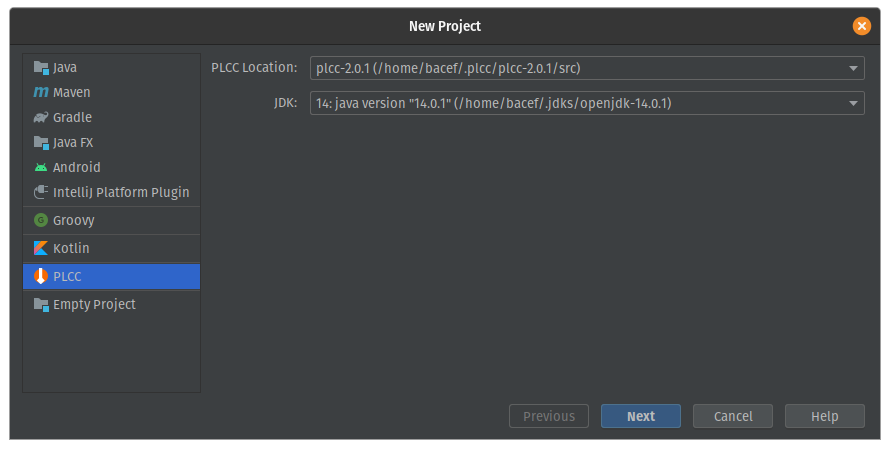
\includegraphics[width=6in]{proj_config.png}
    \caption{New Project creation pop-up with a PLCC project selected. Compilers are autodetected.}
    \label{fig:proj_config}
\end{figure*}

\subsection{Project Creation}\label{subsec:project-creation}
The idiom of creating a new project in Intellij is to work out the details before development should begin.
In this case, our goal is to run an interpreter generated from a .plcc file with .ijava extension files.
Before a .plcc file is compiled and the interpreter is run, both a PLCC compiler and a Java distribution must be installed on the user's computer.
This is because PLCC outputs the interpreter in the form of Java classes.

When a user clicks \textit{File $\rightarrow$ New Project}, they are presented with different project types to choose from on the left side of the new pop-up displayed as seen in figure~\ref{fig:proj_config}.
For the project type that is selected, on the right side there will be some sort of custom GUI that the user can interact with.
The right side of a PLCC project contains two labeled combo boxes, one for the PLCC program location and one for the Java JDK.

\subsubsection{PLCC Program Location Selection}\label{subsubsec:plcc-program-location}
The PLCC dropdown has two default options, plus zero or more other options based on how many PLCC programs are downloaded on a user's computer.
The first default option is to download PLCC\@.
When selected, The PLCC program is downloaded and put in the user's home directory, and an entry for that file is added to the drop-down.
The second default option is to find a PLCC installation on the user's computer.
When clicked, a file picker will open up, so the user is able to pick where the installation is located.
If the selected path has a valid installation, it is added to the drop-down list.
The other options possible are autodetected installations.
Before the drop-down list appears, the \textit{\$HOME/.plcc} directory will be searched for valid installations as well as whatever directory the environment variable LIBPLCC holds.

\subsubsection{JDK Selection}\label{subsubsec:jdk-installation}
The JDK drop-down box will be populated with all the confirmed installations that Intellij has cached throughout the usage of the IDE. Any of these may be selected.
The PLCC output is compatible with Java 7 or higher.

\subsubsection{Generated Project File Structure}\label{subsubsec:generated-project-file-structure}
After \textit{next} is selected and the user selects the directory and name of the project they want to create, they are presented with the editor and project file list.
There will be a directory created under the project directory named \textit{plcc} where the user is expected to store the .plcc file(s) they create.
within that directory, there is a \textit{Java} directory that is marked as sources root.
This is the directory that PLCC will put the generated Java files.
Marking a directory as sources root means that the directory is where Intellij expects to find Java files.

\begin{figure*}[!t]
    \centering
    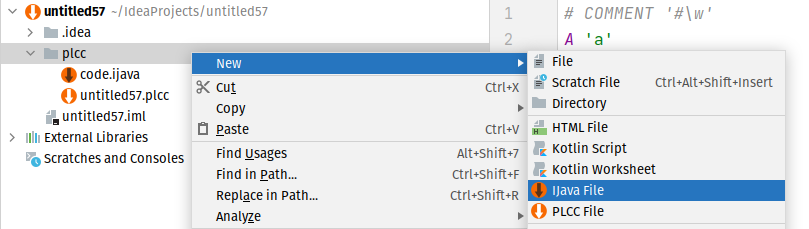
\includegraphics[width=4in]{new_PLCC_file_shortcut.png}
    \caption{Create a new .plcc file. The file will contain the basic syntax structure.}
    \label{fig:new_file_shortcut}
\end{figure*}
\subsection{New File Shortcuts}\label{subsec:new-plcc-file-shortcut}
When a user is ready to develop a .plcc or .ijava file, the creation is easy.
They simply right click on the directory and click \textit{New} and both PLCC and IJava entries show up to be selected.
The new file created will have the file extension according to which option they selected.
It will also contain the basic syntactic framework of one of those files, but with comments where the code needs to go.
This syntax is useful for a new PLCC developer, but may be a burden to familiar PLCC developers.

If a user does not want the new .plcc or .ijava files to have framework code already in there, and they know the correct file extension, they can just create a generic file using \textit{New $\rightarrow$ File} and specifying the name of the file with the extension .plcc or .ijava.
Every file ending with .plcc or .ijava has a unique icon to the left of the title so it can be easily recognised.


\begin{figure*}[!t]
    \centering
    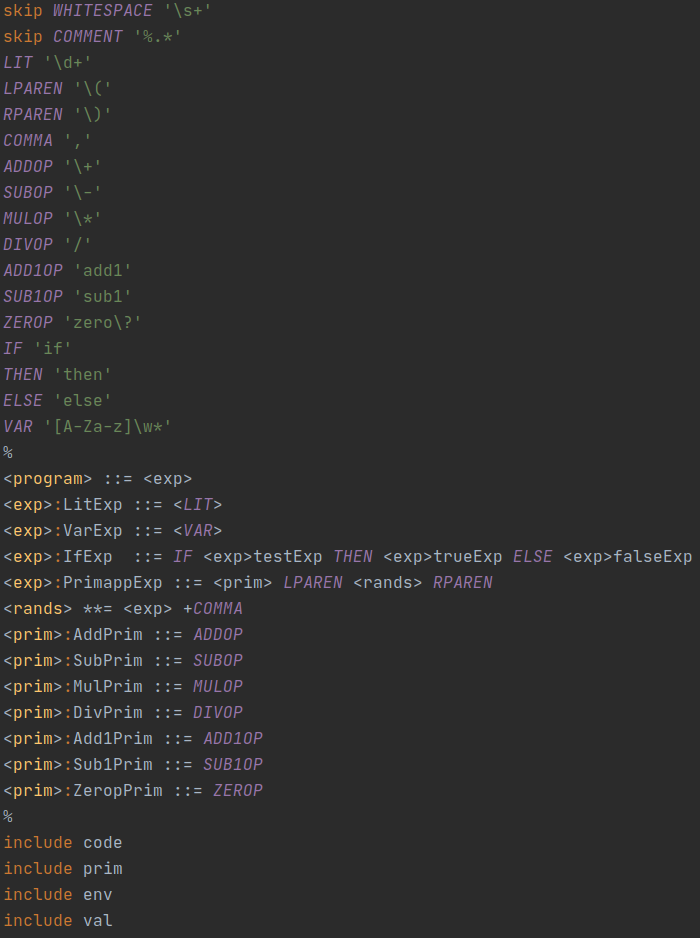
\includegraphics[width=4in]{syntax.png}
    \caption{Syntax highlighting on a valid .plcc file}
    \label{fig:syntax}
\end{figure*}
\begin{figure*}[!t]
    \centering
    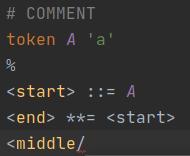
\includegraphics[width=1.5in]{syntax_invalid.png}
    \caption{Syntax highlighting on an invalid  .plcc file. Unexpected characters are underlined in red}
    \label{fig:syntax_invalid}
\end{figure*}

\subsection{Syntax Highlighting}\label{subsec:new-.plcc-file-syntax-highlighting}
Any file with the extension .plcc or .ijava in the project will have its syntax highlighted.

\subsubsection{Syntax Recognising}\label{subsubsec:syntax-recognising}
In order to highlight text in the file, a syntax recogniser needs to be created.
A common way to do this in Intellij is to define a .flex file to tokenize a file, and a .bnf file to parse the file based on the token definitions from the .flex file.
JFlex is the tool that generates a Java token parser from a .flex file.
For the parser, Intellij compiles the grammar rules specified in the .bnf file into Java code as well.
The tokenizer and parser code are then linked up together to create the syntax recogniser.
Intellij does not run the full syntax recogniser every time a file is changed, but uses some reentrant algorithm to keep new code highlighted efficiently.
If the code in the file does not parse, Intellij will put a red underline under the incorrect character(s) and tell the user the token type(s) that were expected in the place of the character.
Valid syntax in an invalid file will still be highlighted.
See figure~\ref{fig:syntax_invalid}.

\subsubsection{Coloring Token Types}\label{subsubsec:coloring-token-types}
In order to make text different colors, token types from the .flex file need to be told what color they should be.
Token types can be assigned a certain color, or a color class that Intellij provides (like \textit{String Literal} or \textit{Identifier}) that will change color according to the UI theme.
If other plugins use these classes for similar token types in their language, and a user has seen syntax in many languages in Intellij, it is easier for them to make out what a specific syntax element is and means.

\subsection{Line Commenting}\label{subsec:line-commenting}
Intellij encourages the line comment keyboard shortcut to be \textit{Ctrl + /}.
The PLCC language has only a line comment character, which is \textit{\#}.
If the cursor is either on a line or if one or more lines are highlighted, when \textit{Ctrl + /} is pressed, all those lines will have a \textit{\#} character prepended to them.


\subsection{PLCC Run Configuration}\label{subsec:plcc-run-configuration}
A Run Configuration template has been created for PLCC\@.
When selected, a GUI is displayed on the right side of the Run Configuration pop up.
The only input necessary from the user is to pick the .plcc file from the text box shown.
If only one .plcc file exists in the plcc directory, it will be autopopulated.

When the run button is clicked with a PLCC run configuration, the Intellij \textit{Run} tab will open and run the PLCC language processor with the .plcc file.
If the .plcc file correctly executed with the PLCC program, the Java files will be generated into a folder named \textit{Java} in the same directory as the .plcc file ran.
Since this \textit{Java} directory was marked as a sources root during project creation, Intellij will recognize these files as Java classes.

If a user wants to see the AST of feeding a snipet of their own language into the interpreter, they would create a simple Java run configuration and run the generated Parse class with possible a file as an argument.
This process is the same for Rep and Scan (Rep starts a REPL, and scan shows the tokens tokenized).
If a user wants to see an AST representation of their language syntax while still running the interpreter, they would add an argument \textit{-t} to Rep.


\section{Conclusion}\label{sec:conclusion}
A PLCC plugin has been implemented with the following features:
\begin{itemize}
    \item Project Setup Wizard to select PLCC location and Java location
    \item New File creation shortcuts for .plcc and .ijava files with basic syntax framework
    \item Syntax recognition and highlighting for .plcc files
    \item Syntax recognition for .ijava files
    \item Keyboard shortcut line commenting
    \item Run Configuration template for a PLCC
\end{itemize}
It is available on the JetBrains Plugin Marketplace under the name "PLCC".
The source code is at \href{https://github.com/ourPLCC/plcc-intellij}{github.com/ourPLCC/plcc-intellij}.

We hypothesize that learning how to use the IDE plugin along with the bugs the user may encounter, will be slightly overpowered by the ease of use the plugin provides over the old development process.
More user research, plugin features as well as plugin development testing could make this an even easier choice.

\subsection{More Proposed Features}\label{subsec:more-proposed-features}

Some future features that could make the development experience better are:
\begin{itemize}
    \item Implementation of Syntax highlighting for Java code within a \%\%\% code block
    \item Many context hints need to be implemented, for example reference and usage highlighting, graying out unused grammar rules, autocompletion of grammar rules and token type definitions, goto .ijava file declaration for grammar rules and include statements, and more.
    \item A run configuration should consist of a user selecting a .plcc file as well as selecting Parse Scan or Rep so that generation, compilation and running happens all at once.
    PLCC will not need to be run if the .plcc file was not changed.
\end{itemize}

%------------------------------------------------------------------------------------
% An example of a floating figure using the graphicx package.
% Note that \label must occur AFTER (or within) \caption.
% For figures, \caption should occur after the \includegraphics.
% Note that IEEEtran v1.7 and later has special internal code that
% is designed to preserve the operation of \label within \caption
% even when the captionsoff option is in effect. However, because
% of issues like this, it may be the safest practice to put all your
% \label just after \caption rather than within \caption{}.
%
% Reminder: the "draftcls" or "draftclsnofoot", not "draft", class
% option should be used if it is desired that the figures are to be
% displayed while in draft mode.
%

%A image is shown in Figure~\ref{fig:myfigure}.
%A citation\cite{IEEEexample:article_typical}.
%
%\begin{figure}[!t]
%    \centering
%    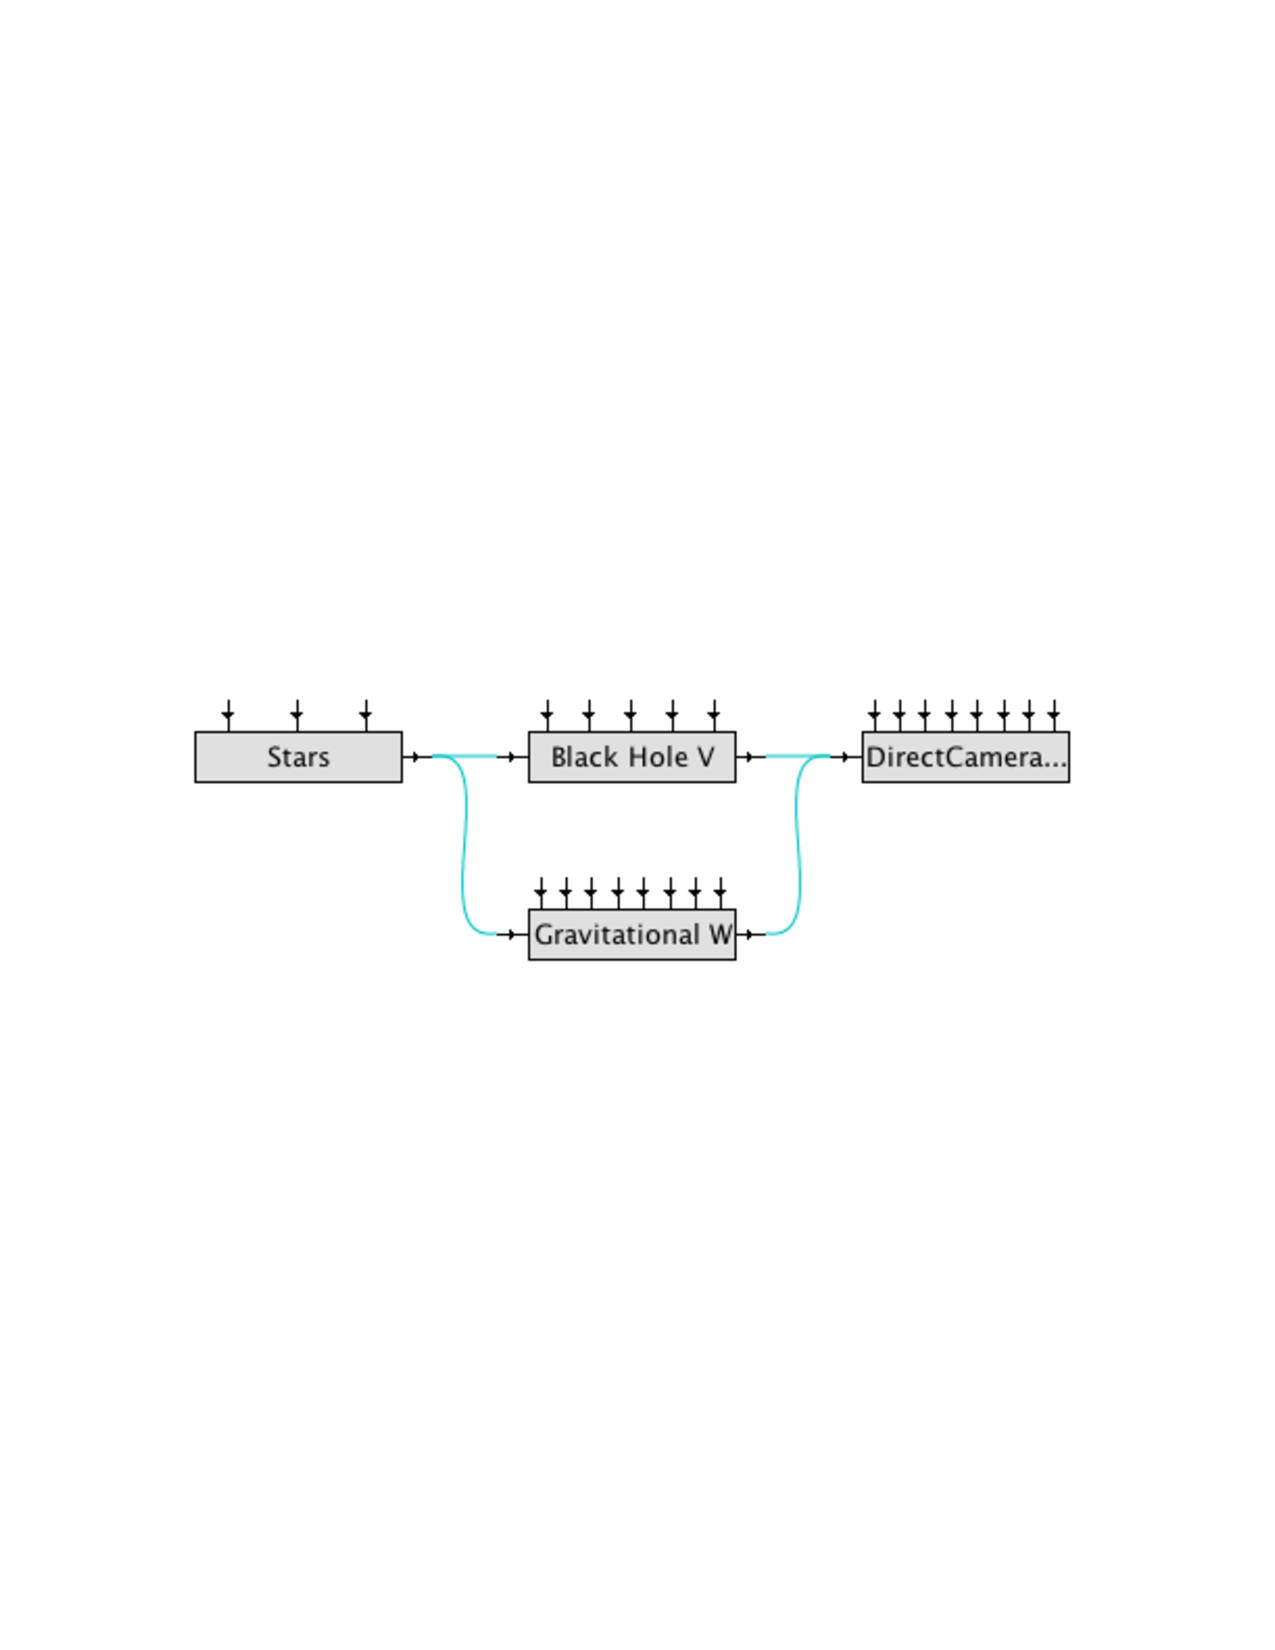
\includegraphics[width=2.5in]{myfigure}
%    % where an .eps filename suffix will be assumed under latex,
%    % and a .pdf suffix will be assumed for pdflatex; or what has been declared
%    % via \DeclareGraphicsExtensions.
%    \caption{Simulation Results}
%    \label{fig:myfigure}
%\end{figure}
%------------------------------------------------------------------------------------


%------------------------------------------------------------------------------------
%In Listing~\ref{hw} a HelloWorld program is shown.
%
%\begin{lstlisting}[caption=writer.c., label=hw]
%int main() {
%  char * msg = "Hello World\n";
%  write(STDIN_FILENO, msg, strlen(msg));
%  exit(0);
%}
%\end{lstlisting}
%------------------------------------------------------------------------------------

% Note that IEEE typically puts floats only at the top, even when this
% results in a large percentage of a column being occupied by floats.


% An example of a double column floating figure using two subfigures.
% (The subfig.sty package must be loaded for this to work.)
% The subfigure \label commands are set within each subfloat command, the
% \label for the overall figure must come after \caption.
% \hfil must be used as a separator to get equal spacing.
% The subfigure.sty package works much the same way, except \subfigure is
% used instead of \subfloat.
%
%\begin{figure*}[!t]
%\centerline{\subfloat[Case I]\includegraphics[width=2.5in]{subfigcase1}%
%\label{fig_first_case}}
%\hfil
%\subfloat[Case II]{\includegraphics[width=2.5in]{subfigcase2}%
%\label{fig_second_case}}}
%\caption{Simulation results}
%\label{fig_sim}
%\end{figure*}
%
% Note that often IEEE papers with subfigures do not employ subfigure
% captions (using the optional argument to \subfloat), but instead will
% reference/describe all of them (a), (b), etc., within the main caption.


% An example of a floating table. Note that, for IEEE style tables, the
% \caption command should come BEFORE the table. Table text will default to
% \footnotesize as IEEE normally uses this smaller font for tables.
% The \label must come after \caption as always.
%
%\begin{table}[!t]
%% increase table row spacing, adjust to taste
%\renewcommand{\arraystretch}{1.3}
% if using array.sty, it might be a good idea to tweak the value of
% \extrarowheight as needed to properly center the text within the cells
%\caption{An Example of a Table}
%\label{table_example}
%\centering
%% Some packages, such as MDW tools, offer better commands for making tables
%% than the plain LaTeX2e tabular which is used here.
%\begin{tabular}{|c||c|}
%\hline
%One & Two\\
%\hline
%Three & Four\\
%\hline
%\end{tabular}
%\end{table}


% Note that IEEE does not put floats in the very first column - or typically
% anywhere on the first page for that matter. Also, in-text middle ("here")
% positioning is not used. Most IEEE journals/conferences use top floats
% exclusively. Note that, LaTeX2e, unlike IEEE journals/conferences, places
% footnotes above bottom floats. This can be corrected via the \fnbelowfloat
% command of the stfloats package.




% conference papers do not normally have an appendix


% use section* for acknowledgement
%\section*{Acknowledgment}
%
%
%The authors would like to thank...





% trigger a \newpage just before the given reference
% number - used to balance the columns on the last page
% adjust value as needed - may need to be readjusted if
% the document is modified later
%\IEEEtriggeratref{8}
% The "triggered" command can be changed if desired:
%\IEEEtriggercmd{\enlargethispage{-5in}}

% references section

% can use a bibliography generated by BibTeX as a .bbl file
% BibTeX documentation can be easily obtained at:
% http://www.ctan.org/tex-archive/biblio/bibtex/contrib/doc/
% The IEEEtran BibTeX style support page is at:
% http://www.michaelshell.org/tex/ieeetran/bibtex/
\bibliographystyle{IEEEtran}
\bibliography{IEEEabrv,example}
% argument is your BibTeX string definitions and bibliography database(s)
%\bibliography{IEEEabrv,../bib/paper}
%
% <OR> manually copy in the resultant .bbl file
% set second argument of \begin to the number of references
% (used to reserve space for the reference number labels box)
% \begin{thebibliography}{1}
% 
% \bibitem{IEEEhowto:kopka}
% H.~Kopka and P.~W. Daly, \emph{A Guide to \LaTeX}, 3rd~ed.\hskip 1em plus
%   0.5em minus 0.4em\relax Harlow, England: Addison-Wesley, 1999.
% 
% \end{thebibliography}




% that's all folks
\end{document}


